\chapter{Calibrating model graders and separating agreement from correctness}\label{calibrating-model-graders-and-separating-agreement-from-correctness}

Two graders that answer PASS on every submission agree on every item. Their agreement is 100 percent and their usefulness is zero. Most submissions in an easy stream really do pass, and neither grader has ever separated a defect from a success.

When the graders are models, that failure is easy to ship. An \textbf{LLM-as-judge} is a model used to grade another system's output. My own migration-evaluation framework gates its two judges on Cohen's kappa rather than on raw agreement, with an agreement floor and a minimum trial count both fixed before any judge ran, because percent agreement overstates judge quality when easy cases dominate the sample. That gate has run against replay fixtures, not against a live evaluation. It illustrates a design decision and does not supply a field result.

The measurement problem arrives before any threshold is chosen. A grader's label can agree with a second grader, match a human label, correspond to an independently checkable outcome, or state a well-calibrated probability. Those are four different properties, and a grader can hold one while failing another. The distinction is lost as soon as the labels are stored as if they were facts.

Chapter 4 set aside the tasks whose correctness execution cannot establish. Model grading supplies a validation lane for some of them, provided the grader itself is treated as an instrument under test. The question is whether its decisions track the judgment the evaluation needs, and it has to be answered before those decisions control releases, rankings, rewards, or training data. The test must run at the class balance and error costs that will exist in operation.

\section{Build the reference labels before the grader}\label{build-the-reference-labels-before-the-grader}

Calibration begins with a \textbf{rubric}, the written scoring criteria a grader applies. Domain experts should write its categories, decision rules, exclusions, and examples, because the resulting labels encode their judgment. A prompt engineer can make the wording consistent. Only someone with the domain knowledge can decide which factual omission is material in a medical summary, or which behavioral mismatch makes a migration unsafe.

Category definitions need to be specific enough that two experts can apply them independently. ``High quality'' leaves the decision inside the rater. ``PASS if every requested behavior is present, no stated constraint is violated, and every factual claim is supported by the supplied record'' names observations that two people can compare. Examples should include boundary cases and counterexamples, especially the cases on which experts initially disagreed.

\subsection{Agreement before automation}\label{agreement-before-automation}

\textbf{Inter-rater reliability} is the degree to which independent raters assign the same labels to the same items. It is a precondition for treating any label set as a reference. If experts cannot apply the categories consistently, a model that reproduces one expert's choices may imitate an unstable convention while appearing to measure the intended property.

Raw percent agreement answers one narrow question. On what share of items did the two labels match? Consider 100 items and two raters who each use PASS 90 times and FAIL 10 times. Suppose they disagree on ten items, with each rater assigning five of those items to each category. Their observed agreement is 90 percent, which looks strong until label prevalence enters the calculation.

Given those marginal label counts, independent assignments would agree on 82 of the 100 items on average. The two 90 percent PASS rates account for 81 expected agreements and the two 10 percent FAIL rates for one. Cohen (\href{https://doi.org/10.1177/001316446002000104}{1960}) defined kappa as the share of the available above-chance agreement that the raters achieved. Here the raters gained eight agreements above an expected 82, out of the 18 above-chance agreements available, which is a kappa of about 0.44.

The always-PASS pair is the degenerate limit of that calculation. Observed and expected agreement are both 100 percent. Kappa is undefined there, because no variation remains from which above-chance agreement could be estimated.

\begin{figure}
\centering
\pandocbounded{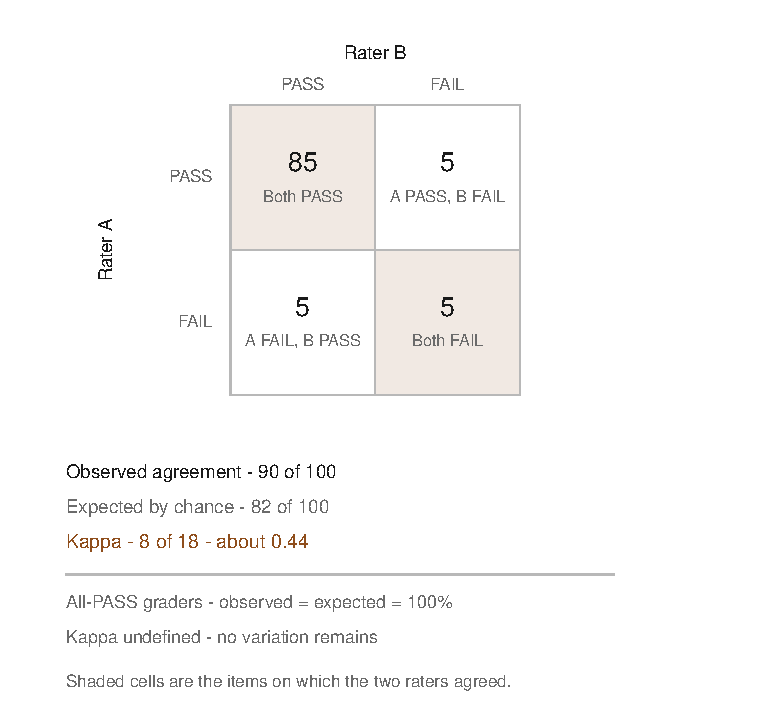
\includegraphics[keepaspectratio,alt={Cells of 85, 5, 5, and 5 produce 90\% observed versus 82\% expected agreement and kappa about 0.44; two always-PASS graders produce 100\% observed and expected agreement but undefined kappa.}]{figures/ch05-agreement-kappa.pdf}}
\caption{Cells of 85, 5, 5, and 5 produce 90\% observed versus 82\% expected agreement and kappa about 0.44; two always-PASS graders produce 100\% observed and expected agreement but undefined kappa.}
\end{figure}

A 100-item example separates observed from chance-corrected agreement; unanimous PASS ratings leave kappa undefined because the ratings contain no variation.

Cohen's kappa handles two raters and computes chance agreement from each rater's observed category frequencies. Fleiss (\href{https://doi.org/10.1037/h0031619}{1971}) extended the chance-corrected idea to several raters and to designs in which different raters label different items. Scott (\href{https://doi.org/10.1086/266577}{1955}) defined a related two-rater measure, Scott's pi, that uses a pooled category distribution when computing chance agreement. None of the three makes an ambiguous rubric reliable. Each makes the ambiguity harder to conceal behind a large agreement percentage.

Because chance agreement is computed from the observed category frequencies, two kappa values estimated under different label prevalences are not directly comparable. A kappa reported without its category distribution is a number without its denominator.

There is no universal kappa threshold that converts labels into truth. The acceptable value depends on the decision, the category prevalence, the number of categories, and the cost of a disagreement. The useful practice is iterative. Experts label the same sample independently, the disagreements are inspected, the category definitions are revised, and the cycle repeats on fresh items. Cemri et al.~(\href{https://arxiv.org/abs/2503.13657}{2025}) ran that sequence with six annotators until Cohen's kappa reached 0.88, and only then tested an automated annotator before using it at scale.

The comparison set must stay outside the grader's development path. A held-out expert-labeled set contains items labeled by domain experts and partitioned away from prompts, examples, fine-tuning data, threshold selection, and any other material the grader could have seen. Orosz and Husain (\href{https://newsletter.pragmaticengineer.com/p/evals}{2025}) describe the same held-out validation and report it through class-specific rates rather than percent agreement, as practitioner experience rather than a controlled result. Row-level random splitting is insufficient when paraphrases, related tasks, or several outputs from the same underlying case cross the boundary. Chapter 3's contamination model applies directly. An answer-bearing example seen during judge construction can make reproduction look like judgment.

Natural sampling produces a second distortion. Suppose a deployment stream contains 950 routine passes, 30 borderline cases, and 20 clear defects per 1,000 items. A random validation sample of 100 items will contain about two clear defects. Missing one of them changes the estimated defect-detection rate by 50 percentage points, while a grader that accepts everything still looks highly accurate.

\textbf{Stratified sampling} fixes the share drawn from each stratum, such as score band, task type, or outcome class. A validation set might draw 40 routine passes, 40 borderline cases, and 40 defects even though those categories occur at very different rates in operation. The design puts enough rare and costly cases under observation to measure them. An aggregate meant to represent deployment must then reweight the strata to the deployment frequencies, because the deliberately balanced sample does not supply that aggregate by itself.

\begin{figure}
\centering
\pandocbounded{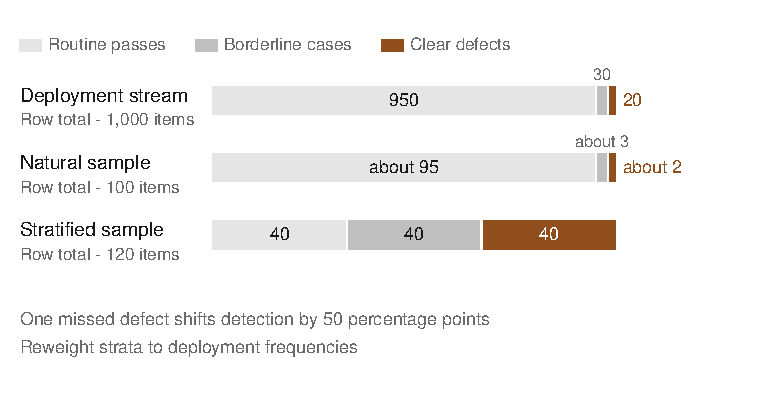
\includegraphics[keepaspectratio,alt={Equal-length bars compare 950 routine, 30 borderline, and 20 defect deployment items with natural 95, 3, and 2 and stratified 40 each requiring reweighting; one missed defect changes detection by 50 percentage points.}]{figures/ch05-sampling-prevalence.pdf}}
\caption{Equal-length bars compare 950 routine, 30 borderline, and 20 defect deployment items with natural 95, 3, and 2 and stratified 40 each requiring reweighting; one missed defect changes detection by 50 percentage points.}
\end{figure}

In a 1,000-item stream, a natural sample expects two clear defects; one miss swings detection by 50 points. Stratified aggregates require deployment reweighting.

How many cases each stratum needs is a power question of the kind Chapter 1 develops. The precision of an estimated detection rate depends on the number of defects in the set, not on the total number of items in it.

Class-specific rates state which error was observed. Treat a defect as the positive class. The true-positive rate, or TPR, is the share of expert-labeled defects that the grader flags. The true-negative rate, or TNR, is the share of expert-labeled nondefects that it accepts. The false-positive rate, or FPR, is the share of nondefects that it flags.

If a set contains 40 defects and 80 nondefects, a grader that catches 32 defects has a TPR of 80 percent. If it also flags 12 of the 80 nondefects, its FPR is 15 percent and its TNR is 85 percent. The operational trade is then explicit. The grader misses 8 defects, and 12 acceptable outputs receive unnecessary review or rejection. One accuracy number merges the two consequences, and it moves when only the class mix changes. TPR, TNR, and FPR are each estimated inside one class, so they do not move with the sampling mix. Because of that invariance, a deliberately balanced validation set can be used to estimate all three rates.

Many judges return a score before a label. The operating point is the threshold together with the error rates the grader produces there. Lowering a defect threshold usually catches more defects and also flags more acceptable work, raising both TPR and FPR. Raising it makes the opposite trade. A grader therefore performs at an operating point under a stated distribution and rubric. It does not have one context-free quality level.

An error budget makes the threshold choice explicit. Suppose reviewers can inspect false alarms on at most 5 percent of acceptable submissions. The evaluator chooses a threshold that holds FPR near that limit and then reports the resulting TPR. ``TPR at a fixed FPR'' names exactly that conditional result.

Threshold selection and final reporting should use separate data, or a design that accounts for the selection. Choosing the best point on the same small set makes the reported rates optimistic.

Those four components are the measuring instrument. Expert agreement tests whether the reference labels have a stable meaning, and the stratified set puts difficult and rare cases under observation. Class-specific rates report the errors that one aggregate accuracy number does not separate. At the operating point, those errors are weighed against the review capacity and failure cost of the deployed system.

\subsection{Calibrate the judge, then scale}\label{calibrate-the-judge-then-scale}

Panthi and Abdelfattah (\href{https://arxiv.org/abs/2605.24060}{2026}) supply a compact example of the full protocol. They had to adjudicate cases in which two systems received the same rank while a downstream rule could still select different winners. They built a three-way rubric and drew a 115-case human-annotated subset from the contested cases, stratified by credited-rank bucket.

The five-rater assessment reached a Fleiss' kappa of 0.83. A panel of one human and four models reached 0.79, and a second human adjudicated a 36-case overlap. Per-model Cohen's kappa against the human labels ran from 0.77 to 0.87. Those measurements established how the judges related to the reference labels before any judge vote entered the larger adjudication.

Singh Thakur et al.~(\href{https://arxiv.org/abs/2406.12624}{2024}) found in separate comparative work that only the largest judges approached human inter-annotator agreement under chance-corrected metrics, and that raw percent agreement concealed systematic leniency and position effects. Judge identity is therefore part of the instrument. Model size alone does not supply an acceptance criterion.

Only after that validation did Panthi and Abdelfattah apply a five-model majority vote at temperature 0 to all 1,902 contested cases. Category construction preceded expert labeling, the validation subset preserved the score bands most likely to expose different errors, and scaling followed measured agreement with the human reference. The authors identified the 115-case set as small, so the reported agreement should not be read as a precise value for every subgroup. Temperature 0 also reduces the variation between repeated votes without removing the run-to-run variation Chapter 1 measured at that setting.

The protocol shows why expert labels should stay visible as measurements. Treating them as `ground truth' would conceal one source of error. Five people can share an interpretation that another qualified group would reject, and adjudication can suppress a disagreement without resolving the ambiguity in the category that produced it. Each rater's original label, the adjudicated label, and the rubric version should be retained, so a later revision can reconstruct which definition produced the result.

Judge validation should also include controlled perturbations, because one aggregate comparison can average away predictable biases. Zheng et al.~(\href{https://arxiv.org/abs/2306.05685}{2023}) documented position, verbosity, and self-preference effects in model judges. To test position sensitivity, present the same response pair in both orders and measure how often the preferred answer changes. Randomizing order during ordinary evaluation reduces the systematic benefit to the first or second position, and the controlled swap estimates how much order still affects the decision.

Leniency appears when a judge accepts work that the rubric marks defective. The probe uses matched cases that differ by one material violation and records the outcome as a class-specific miss. A judge that agrees with experts on routine passes and forgives most subtle defects can hold high aggregate agreement while failing at the decision for which it was added.

Verbosity bias requires a different control. Give the judge semantically equivalent answers whose main difference is irrelevant explanation, or add correct-sounding detail that does not repair the original omission. A preference for the longer response then appears as a label change with no corresponding change in support. The test has to preserve the substantive content as closely as possible. Otherwise length is confounded with information.

Self-preference is a dependence between the judge and the system that produced an answer. A judge may favor phrasing, conventions, or reasoning patterns associated with its own model family. Concealing model identity helps, but stylistic traces can remain. Using judges from different families reduces one source of correlated error and gives the evaluator a comparison, though different branding does not establish independence.

Answer leakage belongs to the contamination problem from Chapter 3. A judge exposed to reference answers, to rubric examples derived from the evaluation cases, or to memorized public solutions can reproduce a preferred label without evaluating the submitted reasoning. The partition must therefore separate underlying tasks, related variants, and individual responses. Li (\href{https://arxiv.org/abs/2502.01534}{2025}) reports the same direction for preference leakage. That work is directional and does not establish how common the effect is across domains or model generations.

Some properties should not reach the model judge at all. If code can determine whether a required file exists, a test passed, a schema is valid, or a named artifact changed, the corresponding assertion should stay deterministic. A model can assess a claim whose meaning requires judgment after those checks run. Replacing exact observations with generated labels adds variance, cost, latency, and an additional failure path without adding information.

Orosz and Husain also prefer binary PASS and FAIL labels when the downstream action is binary. Binary labels force the rubric to locate the release boundary and make TPR, TNR, and FPR directly interpretable. A five-point scale allows raters and judges to use adjacent values inconsistently, and the distance between 2 and 3 is then easily treated as equivalent to the distance between 4 and 5.

The loss of nuance is deliberate and sometimes unacceptable. A writing assistant may need separate judgments for factual support, coverage, and style, because one PASS label cannot locate the failure. The better response is usually several narrowly defined binary claims, each tied to an action. A graded score remains appropriate when the downstream decision genuinely depends on degree and the scale anchors can be applied reliably.

My own trace-annotation tool makes another distinction explicit. Agreement asks whether annotators choose the same categories. Probability calibration asks whether events assigned confidence 0.8 occur about 80 percent of the time. A recorded compatibility failure sits in the data path of that tool. Legacy annotation files receive confidence 1.0 when read, which makes every imported category appear maximally overconfident. The example is narrative, and it locates calibration state across the stored label, its reader, and the annotator's judgment.

After deployment, a human-reviewed sample stays part of the operating loop. The sample needs ordinary cases as well as flagged cases and known boundaries. Reviewing only judge-human disagreements measures the cases in which the monitoring system already detected trouble, and it misses the cases in which the judge and another automated component make the same error.

The ongoing sample estimates whether class-specific rates have moved and supplies new disagreements for rubric repair. It should preserve the deployed threshold and grader version so a rate change can be assigned to a model update, a distribution shift, or a changed scoring rule. Silent replacement of the underlying model breaks that record even when the prompt and the public model name stay constant.

The calibration has to be redone whenever the domain, rubric, response format, or model generation changes. A judge validated on concise code-review summaries has no automatic claim on long incident reports. Adding a finer defect taxonomy changes both the label prevalence and the expert task. Even a prompt change intended only to clarify wording can move the operating point and should be tested against the held-out expert-labeled set.

The result of this process is bounded. Scaled judging reduces the amount of unreviewed error relative to deploying an untested judge. It does not certify that every accepted output is correct, and the expert reference itself contains disagreement. The value is that those errors become observable before the labels control other systems.

\section{What a panel's vote establishes}\label{what-a-panels-vote-establishes}

Bertalanic (\href{https://arxiv.org/abs/2605.00914}{2026}) found an oracle gap of up to 32.3 percentage points between plurality voting and choosing a correct answer already present among the candidates. The candidate set contained a correct answer, but the vote discarded it. That synthesis is exploratory, and no corroborating result is present in the current evidence record, so the figure establishes a reported failure mode. It does not estimate the failure's frequency across panel designs.

A plurality vote among model instances is itself a model oracle. It assigns the label ``selected'' to one candidate and rejects the others. When that choice loses an available correct answer, the failure belongs to grading rather than to optimization. The selection procedure did not identify correctness within the material it was given.

Voting counts endorsements. It does not test the relation between a claim and the evidence that could make the claim true. Five agents can repeat the same nonexistent command-line flag, and four votes will select it over a correct but less familiar alternative. Increasing the panel to nine makes the count more stable while the unsupported premise remains unexamined.

Correlation makes this failure more likely than an independent-voter model suggests. Model instances can share training data, architecture, system prompts, retrieved context, examples, and decoding conventions. They may converge because each reads the same ambiguous instruction the same way. Agreement then measures the strength of a shared dependency, and it is easily mistaken for independent confirmation. Correlated errors also mean the effective number of independent judgments is smaller than the panel size.

Cross-family judges reduce one obvious source of dependence, which is why my own migration-evaluation framework chose them for its dual-judge gate. The design does not prove that their errors are independent. Different families can inherit the same public reference answer, respond to the same leading rubric, or miss the same omitted repository state. Diversity is a control whose effect must be measured.

Selection needs a second criterion beside the vote count. Grounding represents each consequential assertion as a typed claim linked to the material that supports it. A claim about a test result should point to a recorded test execution. A claim about an interface should point to the relevant source or official specification, and a claim about a file change should resolve to the resulting workspace state.

The type determines what evidence can refute the claim. A numeric performance claim may require a result table and its experimental conditions. A causal explanation may remain an interpretation even when every observed event is recorded. A recommendation can be supported by measured failure costs without becoming a factual statement that one design is universally best.

Typing keeps a fluent paragraph from collapsing several evidentiary obligations into one score. Consider a panel assessing a proposed database migration. The answer may contain a syntactically valid statement, a claim that it preserves existing rows, and a claim that rollback is safe under concurrent writes. A parser can check syntax, an execution test can compare rows, and concurrency safety may require a review or an experiment. One popularity count cannot substitute for those different checks.

Grounding also changes what happens when support is absent. The system can retain the candidate, mark a claim unsupported, and route it for review. Without that state, a panel selects a winner from weak evidence because its interface requires one. The stored record should preserve the candidates, ballots, claim support, selected answer, and reason for abstention, so later audits can separate a generation failure from a selection failure.

Abstention is part of the decision rule. A panel should decline to select when support is insufficient, when the vote is unstable, or when the leading answer fails an independent check. That threshold is an operating point and should be chosen on held-out expert-labeled cases according to the cost of a wrong answer and the cost of review. A bare ``three votes wins'' rule embeds a threshold without measuring either cost.

Principled abstention does not require a particular frontier algorithm. Wang (\href{https://arxiv.org/abs/2604.07667}{2026}) combines conformal uncertainty guarantees with social-choice rules. Kamelhar (\href{https://arxiv.org/abs/2604.23366}{2026}) combines grounding with consensus, and Chen et al.~(\href{https://arxiv.org/abs/2309.13007}{2023}) combines deliberation with consensus. The direction reported by all three is useful, and none of them carries a measured result into this chapter. Their operating properties across correlated judges, changing candidate sets, and open-ended tasks are not settled. The supported practice is narrower. Require evidence for the selected claims, measure an abstention rule, and retain an independent correctness check.

Debate and voting still have useful roles. They can produce alternative hypotheses, expose disagreements, and organize a candidate set that would be expensive for one reviewer to generate. The final selection then passes through an oracle appropriate to the claim. Executable behavior goes to execution, structural facts to an exact auditor, and irreducible judgment to a validated human or model grader.

That separation clarifies a common architecture error. Generation, deliberation, and verification may run in the same process, but they serve different purposes and should not share all the same dependencies. If every stage receives the same answer-bearing context and uses models from the same family, the apparent layers are several views of one failure path.

An independent check need not re-evaluate the entire response. It can target the claims whose failure would change the decision. For a code review, that may mean confirming the cited behavior in the changed code and running the named test. For a research synthesis, it may mean resolving the primary source behind each load-bearing factual statement and abstaining when the source does not support the wording.

Panels also create operational costs that one aggregate score does not show. More judges increase inference expense and latency. Grounding adds retrieval and evidence storage, and abstention transfers work to people or to a slower verifier. Those costs are justified when the avoided false decision is more expensive, and excessive when a deterministic assertion can answer the question directly.

The always-PASS pair from the opening is the degenerate panel. A larger group of correlated judges is the expensive version of the same mistake, when each member repeats the majority class or the same unsupported answer. Perfect internal agreement establishes only that the selection mechanism is stable. Correctness still requires a relation to evidence outside the vote.

The companion catalog carries two narrower controls for readers implementing this architecture: keep an exact auditor beside heuristic graders, and combine judge labels with a human-labeled subset. Each addresses a narrower problem than the core decisions developed in this chapter.

\section{Rebuild the grader as a measured system}\label{rebuild-the-grader-as-a-measured-system}

Begin by deleting any assumption that the current judge prompt defines the target. The people whose judgment the system is meant to encode write the categories and apply them independently to fresh cases. Their disagreements identify missing rules, conflicting interpretations, and tasks that should permit abstention. Revision continues until the measured reliability is adequate for the decision, with the chosen standard and the remaining disagreements both recorded.

The resulting expert-labeled set stays outside judge development and holds enough cases from each consequential score band, task type, and outcome class. Related tasks and answer variants stay on one side of the partition, so contamination cannot cross through paraphrase or shared provenance. Deterministic assertions run separately and remove the claims that code can decide without a model.

Score the candidate judge with chance-corrected agreement and class-specific rates at the threshold intended for deployment. Raw percent agreement stays descriptive rather than becoming the acceptance gate. Report the TPR, TNR, and FPR, the class mix, the sample size within each stratum, and the operating cost that selected the threshold.

Controlled swaps test whether position changes the decision. Matched concise and padded answers expose verbosity preference, and defect pairs measure leniency. Concealed source identity and cross-family comparisons probe self-preference and shared error. These tests belong in the grader's release suite, because a new model generation can change them without any change to the rubric.

Binary decisions keep the boundary legible when the action is pass or fail. Several narrow binary labels preserve more diagnostic information than one vague ordinal score, at the cost of more expert labeling and more judge calls. A genuinely graded decision can keep a score once its anchors and its probability calibration have been tested.

Deployment continues to send a sample through human review. That sample must include unflagged ordinary work together with disputed and rejected cases, or silent false negatives stay absent from the monitoring data. Each record keeps the grader version, rubric version, threshold, model output, human label, and the evidence needed to reproduce the decision.

For a panel, keep the candidates and the ballots, and do not treat plurality as verification. Judges from different families reduce shared model-specific errors. The winning answer still has to carry grounded, typed claims, pass the independent checks available for those claims, and abstain when support falls below the validated operating point.

A change of domain, rubric, format, or model generation reopens all of this work. CodeProbe (\href{https://github.com/sjarmak/codeprobe}{public repository}) contains a dual-curator calibration gate that has not been satisfied, because the qualifying corpus does not yet exist. The code shipped before the corpus. That is calibration debt, and naming it here does not discharge it, so the gate stays unmet until the instrument can be built.

The first build need not be the full corpus. One rubric category and a handful of expert-labeled cases from the score band where that decision turns is enough to begin. The cases must be held out from both the judge prompt and threshold selection, then scored at the threshold intended for deployment and reported as class-specific rates rather than percent agreement. That stratum tests one grading decision and shows which category to label next, while the broader gate stays unmet.

\section{Sources and evidence}\label{sources-and-evidence}

The evidence class and strength on each entry below come from its catalog record. Author-system cases in this chapter are narrative illustration and are not part of the evidence base.

\subsection{Calibrate LLM judges}\label{calibrate-llm-judges}

\begin{itemize}
\tightlist
\item
  explorer/strong: Zheng et al.~(2023), ``Judging LLM-as-a-Judge with MT-Bench and Chatbot Arena,'' arXiv:2306.05685. Judge position, verbosity, and self-preference bias; inter-rater agreement against human labels.
\item
  lit/strong: Singh Thakur, Choudhary, Ramayapally, Vaidyanathan \& Hupkes (2024), ``Judging the Judges,'' arXiv:2406.12624. Chance-corrected alignment metrics, systematic leniency, and position effects.
\item
  lit/strong: Cemri, M., et al.~(2025), ``Why Do Multi-Agent LLM Systems Fail?,'' arXiv:2503.13657. Kappa 0.88 expert taxonomy before validated automated annotation.
\item
  practitioner/directional: Orosz with Husain (2025), ``A pragmatic guide to LLM evals for devs,'' Pragmatic Engineer newsletter, 2025-12-02, \url{https://newsletter.pragmaticengineer.com/p/evals}. Binary PASS/FAIL, deterministic evaluation where possible, and judge validation against held-out human labels with TPR/TNR.
\item
  explorer/strong: Panthi \& Abdelfattah (2026), ``Same Ranking, Different Winner,'' arXiv:2605.24060. The 115-case stratified validation protocol, agreement measurements, overlap adjudication, and scaled contested-case evaluation.
\item
  explorer/directional: Li (2025), ``Preference Leakage,'' arXiv:2502.01534. Direction only.
\item
  explorer/directional: Badagi (2026), ``AI Assurance,'' arXiv:2605.23459. Direction only.
\item
  explorer/directional: ``MemConflict,'' arXiv:2605.20926. Direction only.
\item
  reference/standard method: Cohen, J. (1960). A Coefficient of Agreement for Nominal Scales. Educational and Psychological Measurement 20(1), 37-46. DOI: 10.1177/001316446002000104. Primary source for Cohen's kappa, the agreement statistic the chapter defines; a standard method rather than a catalog evidence item.
\item
  reference/standard method: Fleiss, J. L. (1971). Measuring Nominal Scale Agreement Among Many Raters. Psychological Bulletin 76(5), 378-382. DOI: 10.1037/h0031619. Primary source for Fleiss's kappa, the agreement statistic the chapter defines; a standard method rather than a catalog evidence item.
\item
  reference/standard method: Scott, W. A. (1955). Reliability of Content Analysis: The Case of Nominal Scale Coding. Public Opinion Quarterly 19(3), 321-325. DOI: 10.1086/266577. Primary source for Scott's pi, the agreement statistic the chapter defines; a standard method rather than a catalog evidence item.
\end{itemize}

\subsection{Separate agreement from correctness}\label{separate-agreement-from-correctness}

\begin{itemize}
\tightlist
\item
  explorer/strong: Bertalanic (2026), ``Cost of Consensus,'' arXiv:2605.00914. Oracle gap up to 32.3 percentage points; plurality voting discards correct answers already present; grounding catches failures that agreement masks.
\item
  explorer/directional: Kamelhar (2026), GSAR grounded consensus, arXiv:2604.23366. Direction only.
\item
  explorer/directional: Wang (2026), ``Conformal Social Choice,'' arXiv:2604.07667. Direction only.
\item
  explorer/directional: Chen et al.~(2023), ``ReConcile,'' arXiv:2309.13007. Direction only.
\item
  Corroboration: none on record.
\end{itemize}

\subsection{Author artifact cited inline}\label{author-artifact-cited-inline}

\begin{itemize}
\tightlist
\item
  Not an evidence item: CodeProbe, the author's task-mining evaluation tool, \href{https://github.com/sjarmak/codeprobe}{public repository}. Named inline for the dual-curator calibration gate described in the closing section, which is narrative illustration.
\end{itemize}
